\documentclass[10pt]{beamer}
\usepackage[english]{babel}
\usepackage[utf8]{inputenc}
\usepackage[T1]{fontenc}
\usepackage{helvet}

%-------------------------------------------------------
% INFORMATION IN THE TITLE PAGE
%-------------------------------------------------------


%Principales estrategias y métodos basados en deep learning para la detección de neo antígenos en el marco del desarrollo de vacunas personalizadas en la inmunoterapia del cáncer

\newcommand{\cstitle}{\textbf{ Neoantigen Detection Using Transformers and Transfer Learning \vspace{1cm}}}
\subtitle[]{Universidad La Salle}
\newcommand{\cscourseCode}{Jornadas de Investigación}
\newcommand{\csauthor}{Ph.D(c). Vicente Machaca Arceda}
\institute[UNSA]{Universidad de Ingeniería y Tecnología}
\newcommand{\csemail}{vmachaca@utec.edu.pe}
\newcommand{\instituteabr}{UTEC}
\newcommand{\nameUp}{}
\date{2022-I}
\title[\cscourseCode]{\cstitle}
\author{\csauthor}
%%%%%%%%%%%%%%%%%

%-------------------------------------------------------
% CHOOSE THE THEME
%-------------------------------------------------------
\def\mycmd{0} % UNSA
\def\mycmd{1} % SALLE
\def\mycmd{2} % UTEC
\def\mycmd{3} % SALLE NEW
%-------------------------------------------------------

\if\mycmd0
\usepackage{csformat}
\newcommand{\chref}[3][blue]{\href{#2}{\color{#1}{#3}}}%

\fi

\if\mycmd1
\usetheme[]{Feather}
\newcommand{\chref}[2]{	\href{#1}{{\usebeamercolor[bg]{Feather}#2}} }
\fi

\if\mycmd2
\usetheme{UTEC2020}	
\newcommand{\chref}[3][blue]{\href{#2}{\color{#1}{#3}}}%
\fi

\if\mycmd3
\usetheme[]{SALLE}
\newcommand{\chref}[2]{	\href{#1}{{\usebeamercolor[bg]{Feather}#2}} }
\fi


\newcommand{\1}{
	\setbeamertemplate{background}{
		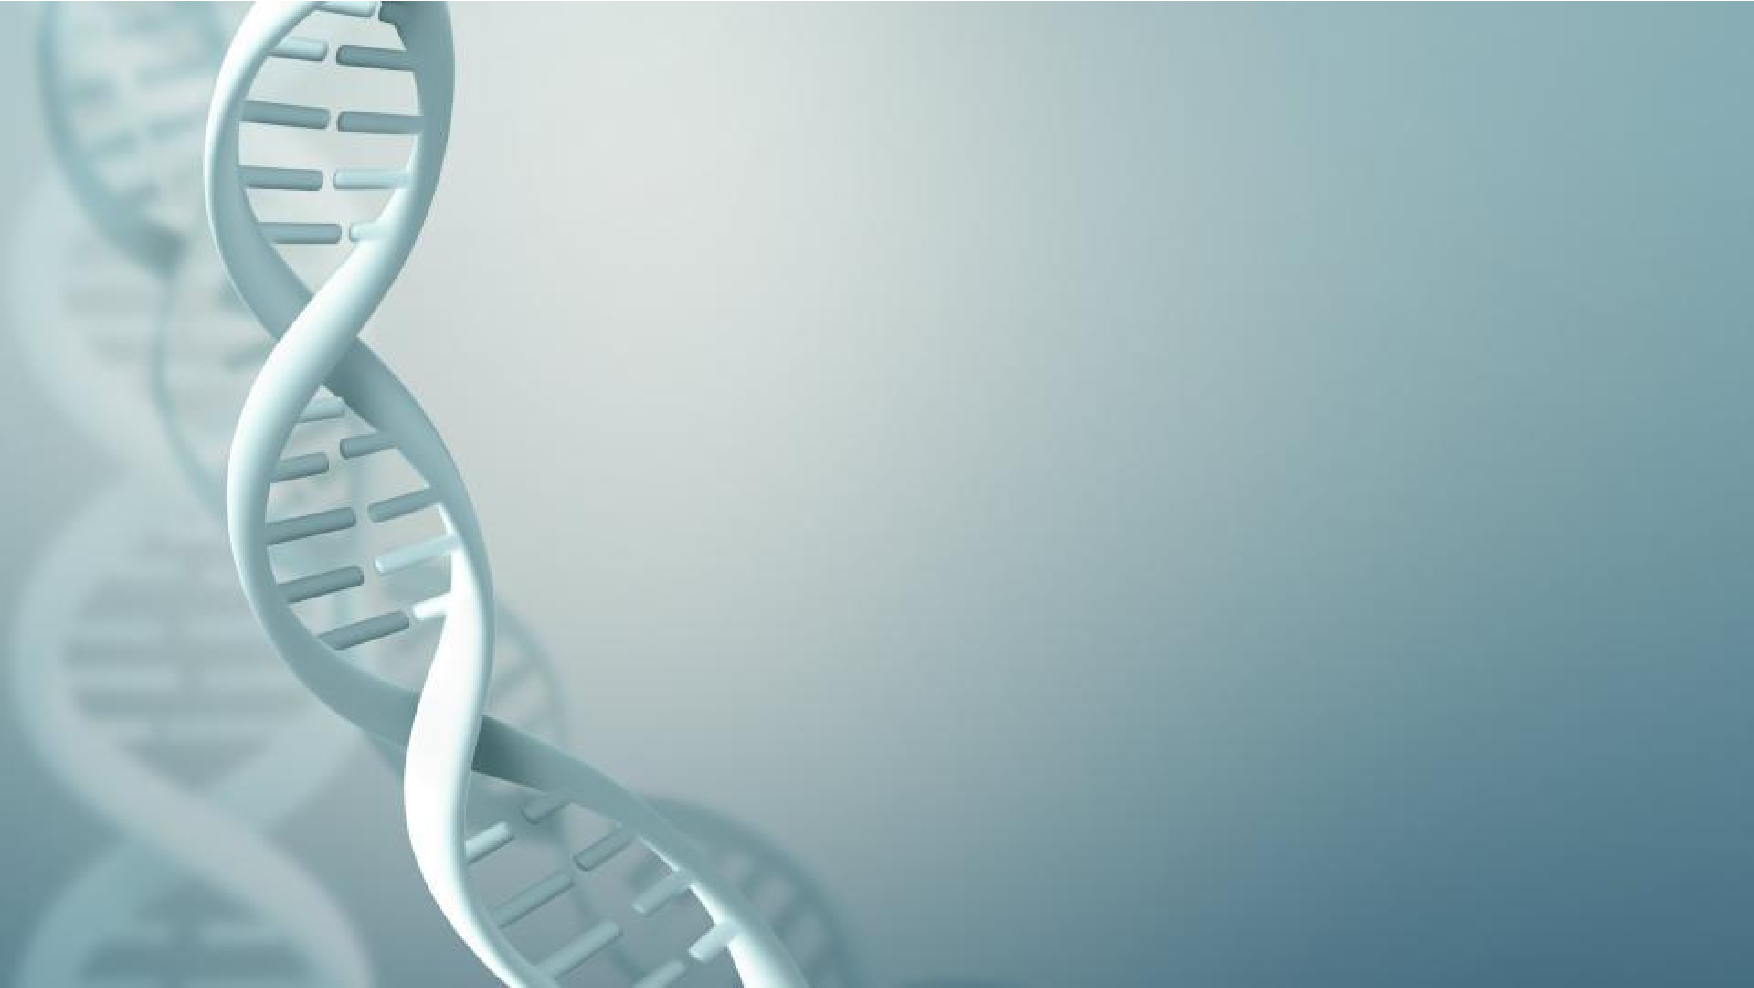
\includegraphics[width=\paperwidth,height=\paperheight]{../img/1}
		\tikz[overlay] \fill[fill opacity=0.75,fill=white] (0,0) rectangle (-\paperwidth,\paperheight);
	}
}



%-------------------------------------------------------
% THE BODY OF THE PRESENTATION
%-------------------------------------------------------

\begin{document}
	
	
	\AtBeginSubsection[]
	{
		\begin{frame}
			\frametitle{Content}
			\tableofcontents[currentsubsection]
		\end{frame}
	}
	
	
	%-------------------------------------------------------
	% THE TITLEPAGE
	%-------------------------------------------------------
	
	\if\mycmd0
	\maketitle
	\fi
	
	\if\mycmd1 % MY THEME
	\1{
		\begin{frame}[plain,noframenumbering] 
			\titlepage 
	\end{frame}}
	\fi
	
	\if\mycmd2
	\begin{frame}
		\titlepage
	\end{frame}
	\fi
	
	\if\mycmd3
	%\titlepage
	\begin{frame}[plain,noframenumbering] 
		\titlepage
	\end{frame}
	\fi
	%-------------------------------------------------------
	%-------------------------------------------------------
	
	
	%-------------------------------------------------------
	%-------------------------------------------------------
	\begin{frame}{Content}
		\tableofcontents
	\end{frame}
	%-------------------------------------------------------
	%-------------------------------------------------------
	
	
	

	
	%%%%%%%%%%%%%%%%%%%%%%%%%%%%%%%%%%%%%%%%%%%%%%%%%%%%%%%%%%%%%%%%%%%%%%%%%%%%%%%%%%%%%%%%%%%%%%%%%%%%%%%%%%%%%%%%
	%%%%%%%%%%%%%%%%%%%%%%%%%%%%%%%%%%%%%%%%%%%%%%%%%%%%%%%%%%%%%%%%%%%%%%%%%%%%%%%%%%%%%%%%%%%%%%%%%%%%%%%%%%%%%%%%
	%%%%%%%%%%%%%%%%%%%%%%%%%%%%%%%%%%%%%%%%%%%%%%%%%%%%%%%%%%%%%%%%%%%%%%%%%%%%%%%%%%%%%%%%%%%%%%%%%%%%%%%%%%%%%%%%
	\section{Introduction}
	%%%%%%%%%%%%%%%%%%%%%%%%%%%%%%%%%%%%%%%%%%%%%%%%%%%%%%%%%%%%%%%%%%%%%%%%%%%%%%%%%%%%%%%%%%%%%%%%%%%%%%%%%%%%%%%%
	%%%%%%%%%%%%%%%%%%%%%%%%%%%%%%%%%%%%%%%%%%%%%%%%%%%%%%%%%%%%%%%%%%%%%%%%%%%%%%%%%%%%%%%%%%%%%%%%%%%%%%%%%%%%%%%%
	%%%%%%%%%%%%%%%%%%%%%%%%%%%%%%%%%%%%%%%%%%%%%%%%%%%%%%%%%%%%%%%%%%%%%%%%%%%%%%%%%%%%%%%%%%%%%%%%%%%%%%%%%%%%%%%%
	
	
	%%%%%%%%%%%%%%%%%%%%%%%%%%%%%%%%%%%%%%%%%%%%%%%%%%%%%%%%%%%%%%%%%%%%%%%%%%%%%%%%%%%%%%%%%%%%%%%%%%%%%%%%%%%%%%%%
	%%%%%%%%%%%%%%%%%%%%%%%%%%%%%%%%%%%%%%%%%%%%%%%%%%%%%%%%%%%%%%%%%%%%%%%%%%%%%%%%%%%%%%%%%%%%%%%%%%%%%%%%%%%%%%%%
	%%%%%%%%%%%%%%%%%%%%%%%%%%%%%%%%%%%%%%%%%%%%%%%%%%%%%%%%%%%%%%%%%%%%%%%%%%%%%%%%%%%%%%%%%%%%%%%%%%%%%%%%%%%%%%%%
	\subsection{Immunotherapy to Treat Cancer}
	%%%%%%%%%%%%%%%%%%%%%%%%%%%%%%%%%%%%%%%%%%%%%%%%%%%%%%%%%%%%%%%%%%%%%%%%%%%%%%%%%%%%%%%%%%%%%%%%%%%%%%%%%%%%%%%%
	%%%%%%%%%%%%%%%%%%%%%%%%%%%%%%%%%%%%%%%%%%%%%%%%%%%%%%%%%%%%%%%%%%%%%%%%%%%%%%%%%%%%%%%%%%%%%%%%%%%%%%%%%%%%%%%%
	%%%%%%%%%%%%%%%%%%%%%%%%%%%%%%%%%%%%%%%%%%%%%%%%%%%%%%%%%%%%%%%%%%%%%%%%%%%%%%%%%%%%%%%%%%%%%%%%%%%%%%%%%%%%%%%%
	
	%-------------------------------------------------------
	%-------------------------------------------------------
	\begin{frame}{Immunotherapy to Treat Cancer}{}		
		Immunotherapy is a type of cancer treatment that helps your immune system fight cancer \cite{inmunoterapy2022}.
		
		\begin{figure}
			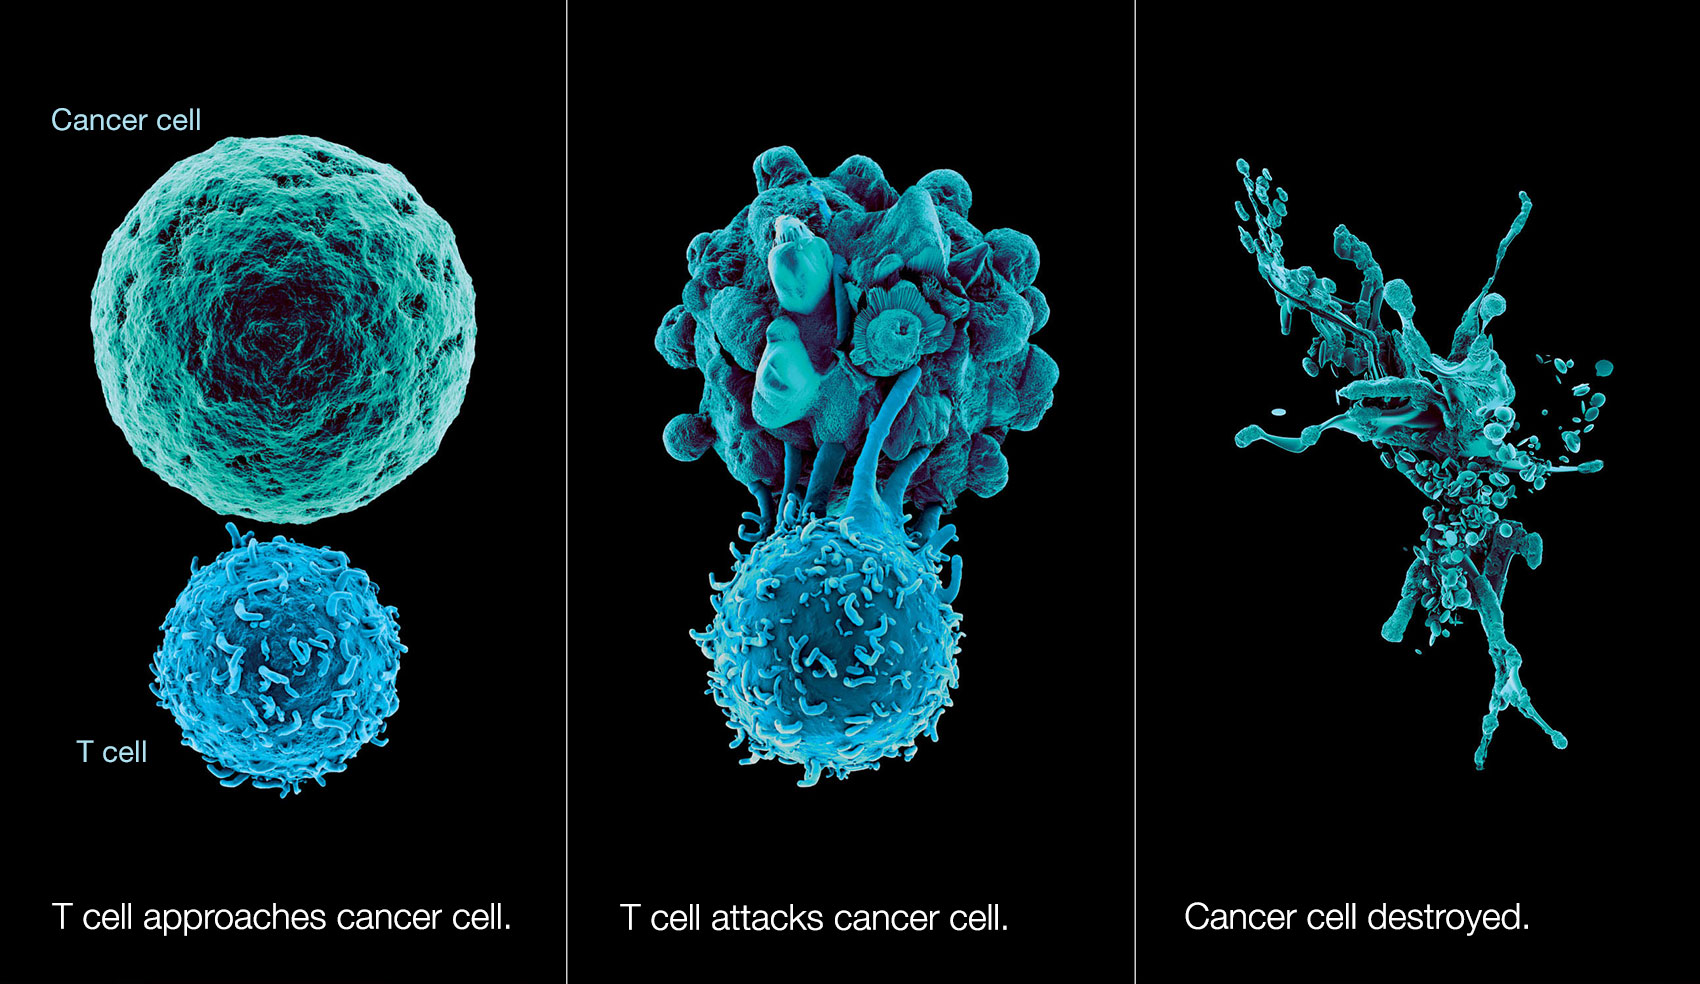
\includegraphics[width=0.7\textwidth]{../img/neoantigen/tcell}
			\caption{Example of how a T cell attack a cancer cell \cite{nortshore2022}.}
		\end{figure}		
	\end{frame}
	%-------------------------------------------------------
	%-------------------------------------------------------
	
	%-------------------------------------------------------
	%-------------------------------------------------------
	\begin{frame}{Immunotherapy to Treat Cancer}{Neoantigen}		
		\begin{block}{Neoantigen}
			A new protein that forms on cancer cells when certain mutations occur in tumor DNA. Neoantigens used in vaccines and other types of immunotherapy are being studied in the treatment of many types of cancer \cite{NCIdictionary2022, borden2022cancer}.
		\end{block} 
		\begin{block}{}
			Currently, there is a lot of methods to detect neoantigens; however, only a small number of them manage to stimulate the immune system \cite{chen2021challenges, hao2021improvement}.
		\end{block}
	\end{frame}
	%-------------------------------------------------------
	%-------------------------------------------------------
	
	
	%-------------------------------------------------------
	%-------------------------------------------------------
	\begin{frame}{Immunotherapy for Cancer}{Personalized Vaccines}	
		\begin{figure}
			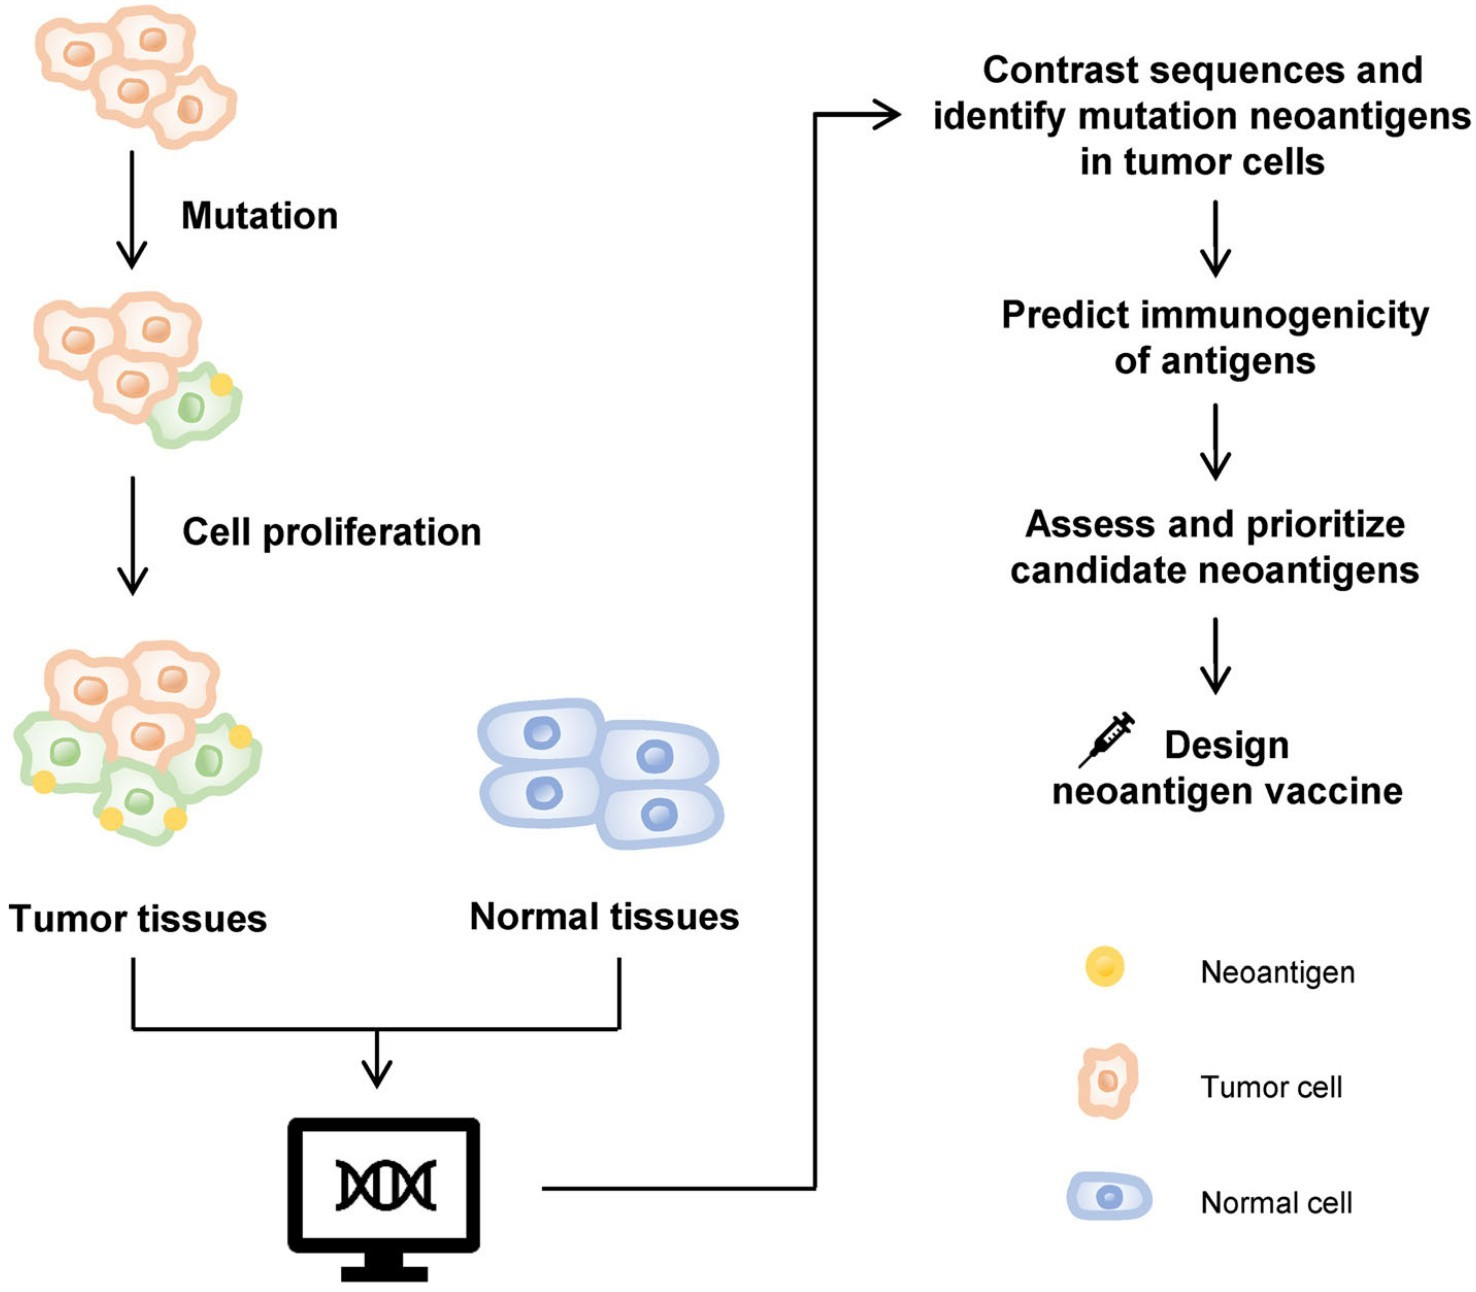
\includegraphics[width=0.6\textwidth]{../img/neoantigen/process}
			\caption{Personalized vaccines process for Cancer \cite{peng2019neoantigen}.}
		\end{figure}		
	\end{frame}
	%-------------------------------------------------------
	%-------------------------------------------------------
	
	%-------------------------------------------------------
	%-------------------------------------------------------
	\begin{frame}{Immunotherapy for Cancer}{Personalized Vaccines}	
		\begin{figure}
			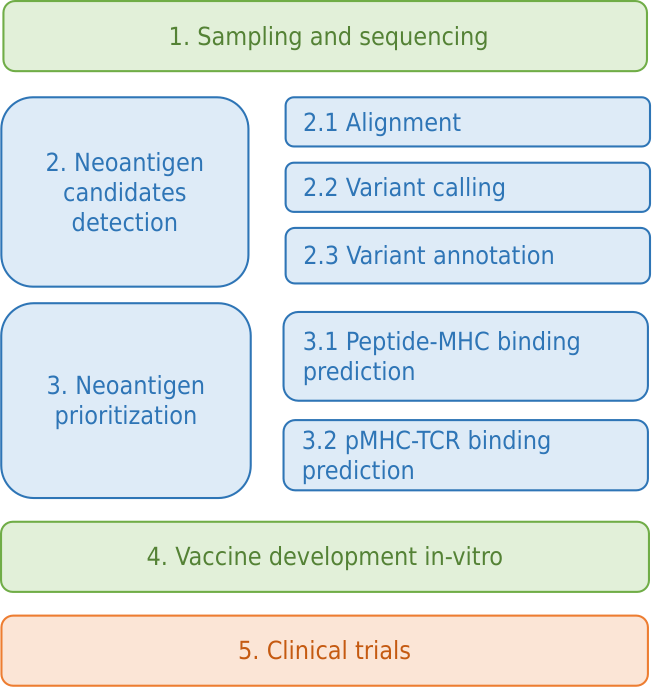
\includegraphics[width=0.6\textwidth]{../img/pipeline/pipeline_ingles}
			\caption{Personalized vaccines process for Cancer.}
		\end{figure}		
	\end{frame}
	%-------------------------------------------------------
	%-------------------------------------------------------
	
	
	
	%-------------------------------------------------------
	%-------------------------------------------------------
	\begin{frame}{pMHC binding prediction}{}		
		\begin{figure}[H]
			\centering
			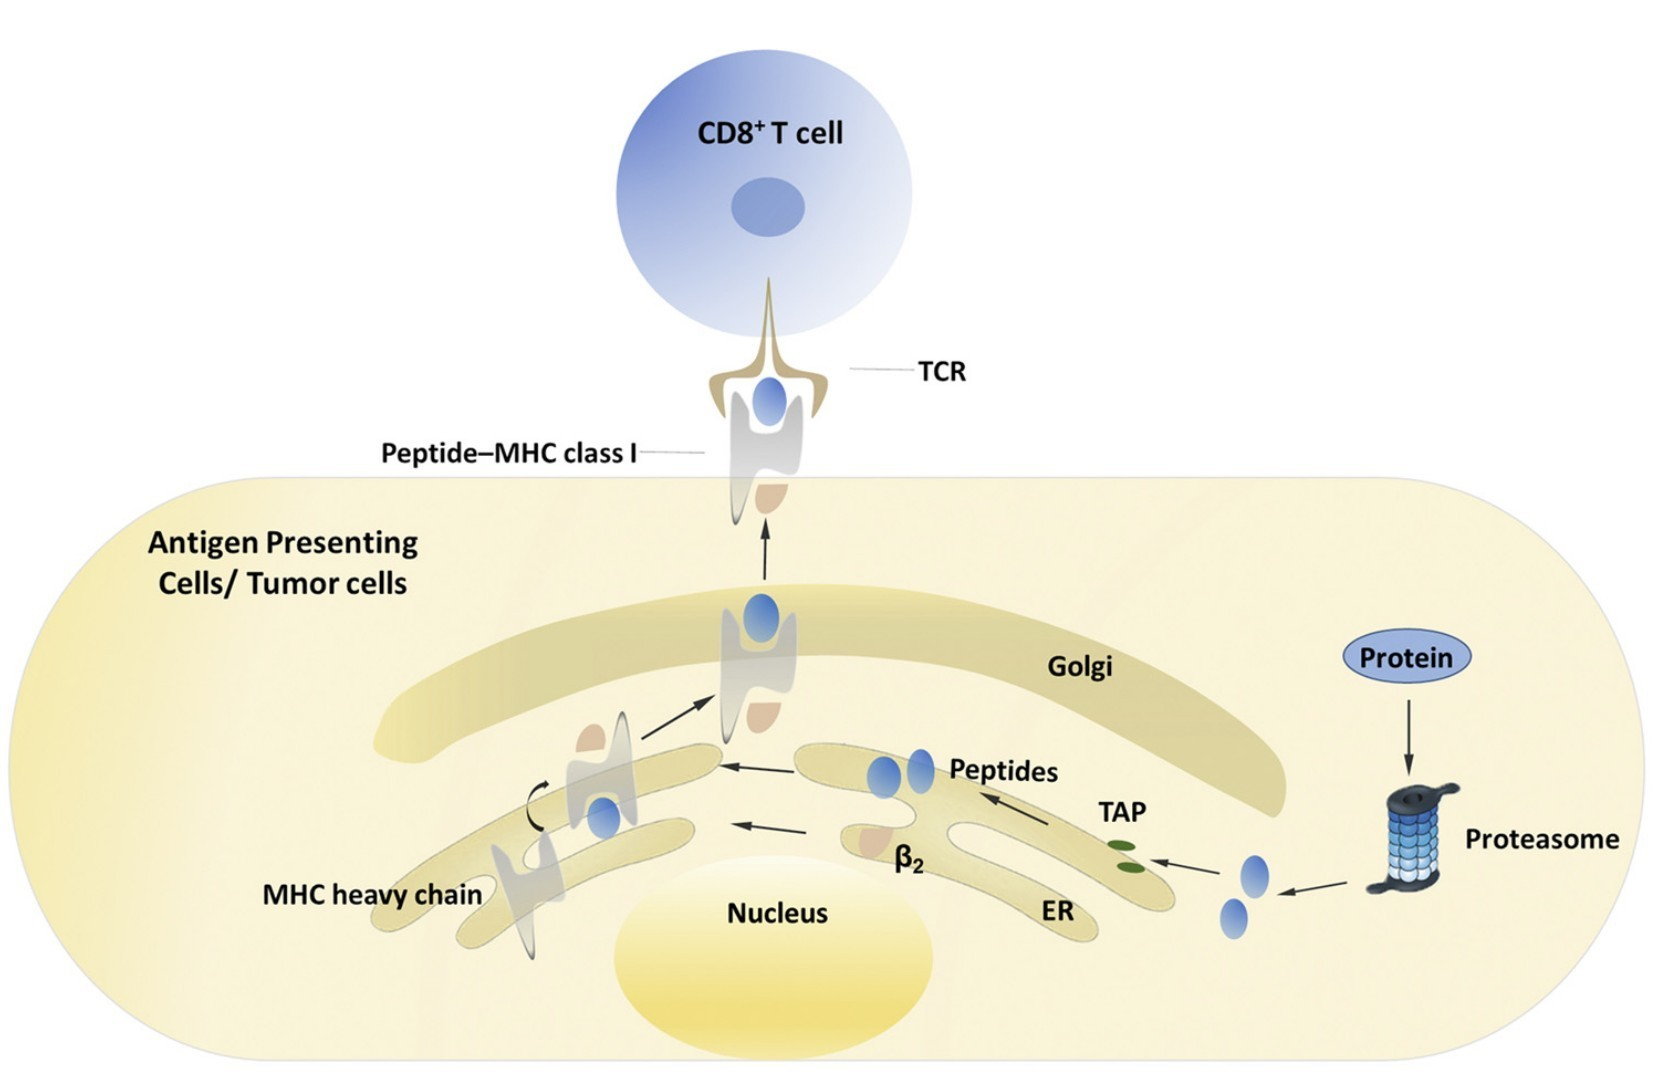
\includegraphics[width=0.8\textwidth]{../img/neoantigen/mhc1.jpg}
			\caption{pMHC presentation process in MHC class I \cite{zhang2019application}.}
			\label{fig:mhc1}
		\end{figure}	
	\end{frame}
	%-------------------------------------------------------
	%-------------------------------------------------------
	
	%%%%%%%%%%%%%%%%%%%%%%%%%%%%%%%%%%%%%%%%%%%%%%%%%%%%%%%%%%%%%%%%%%%%%%%%%%%%%%%%%%%%%%%%%%%%%%%%%%%%%%%%%%%%%%%%
	%%%%%%%%%%%%%%%%%%%%%%%%%%%%%%%%%%%%%%%%%%%%%%%%%%%%%%%%%%%%%%%%%%%%%%%%%%%%%%%%%%%%%%%%%%%%%%%%%%%%%%%%%%%%%%%%
	%%%%%%%%%%%%%%%%%%%%%%%%%%%%%%%%%%%%%%%%%%%%%%%%%%%%%%%%%%%%%%%%%%%%%%%%%%%%%%%%%%%%%%%%%%%%%%%%%%%%%%%%%%%%%%%%
	\subsection{Problem}
	%%%%%%%%%%%%%%%%%%%%%%%%%%%%%%%%%%%%%%%%%%%%%%%%%%%%%%%%%%%%%%%%%%%%%%%%%%%%%%%%%%%%%%%%%%%%%%%%%%%%%%%%%%%%%%%%
	%%%%%%%%%%%%%%%%%%%%%%%%%%%%%%%%%%%%%%%%%%%%%%%%%%%%%%%%%%%%%%%%%%%%%%%%%%%%%%%%%%%%%%%%%%%%%%%%%%%%%%%%%%%%%%%%
	%%%%%%%%%%%%%%%%%%%%%%%%%%%%%%%%%%%%%%%%%%%%%%%%%%%%%%%%%%%%%%%%%%%%%%%%%%%%%%%%%%%%%%%%%%%%%%%%%%%%%%%%%%%%%%%%
	
	%-------------------------------------------------------
	%-------------------------------------------------------
	\begin{frame}{Problem}{Peptide-MHC Binding Prediction}
		
		\begin{block}{}
			\textbf{Less than 5\%} of detected neoantigens (peptides binded to MHC) succeed in activating the immune system \cite{de2020neoantigen}.
		\end{block}
		
		
		\begin{block}{}
			This is a \textbf{binary classification problem}. A peptide could be represented like: $p = \{ A, ... , Q \}$ and a MHC like: $q = \{ A, N, ... ,Q, E \}$. Finally, we need to know the probability of affinity between $p$ and $q$ (pMHC)
		\end{block}
		
		%	\begin{block}{Objectives}
			%		Proposed a method based on transformers and transfer learning for pMHC binding and	presentation prediction. 
			%	\end{block}	
		
	\end{frame}
	%-------------------------------------------------------
	%-------------------------------------------------------
	
	%-------------------------------------------------------
	%-------------------------------------------------------
	\begin{frame}{Problem}{}	
		\begin{figure}
			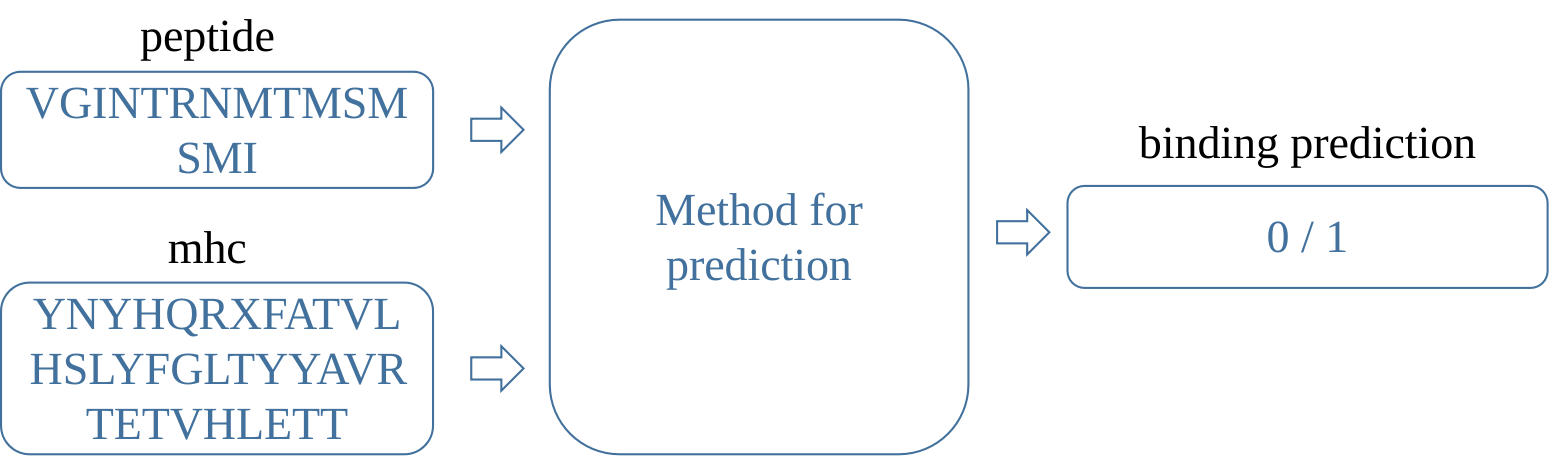
\includegraphics[width=0.9\textwidth]{../img/neoantigen/problem}
			\caption{pMHC binding prediction problem.}
		\end{figure}
	\end{frame}
	%-------------------------------------------------------
	%-------------------------------------------------------
	
	
		%%%%%%%%%%%%%%%%%%%%%%%%%%%%%%%%%%%%%%%%%%%%%%%%%%%%%%%%%%%%%%%%%%%%%%%%%%%%%%%%%%%%%%%%%%%%%%%%%%%%%%%%%%%%%%%%
	%%%%%%%%%%%%%%%%%%%%%%%%%%%%%%%%%%%%%%%%%%%%%%%%%%%%%%%%%%%%%%%%%%%%%%%%%%%%%%%%%%%%%%%%%%%%%%%%%%%%%%%%%%%%%%%%
	%%%%%%%%%%%%%%%%%%%%%%%%%%%%%%%%%%%%%%%%%%%%%%%%%%%%%%%%%%%%%%%%%%%%%%%%%%%%%%%%%%%%%%%%%%%%%%%%%%%%%%%%%%%%%%%%
	\section{Development}
	%%%%%%%%%%%%%%%%%%%%%%%%%%%%%%%%%%%%%%%%%%%%%%%%%%%%%%%%%%%%%%%%%%%%%%%%%%%%%%%%%%%%%%%%%%%%%%%%%%%%%%%%%%%%%%%%
	%%%%%%%%%%%%%%%%%%%%%%%%%%%%%%%%%%%%%%%%%%%%%%%%%%%%%%%%%%%%%%%%%%%%%%%%%%%%%%%%%%%%%%%%%%%%%%%%%%%%%%%%%%%%%%%%
	%%%%%%%%%%%%%%%%%%%%%%%%%%%%%%%%%%%%%%%%%%%%%%%%%%%%%%%%%%%%%%%%%%%%%%%%%%%%%%%%%%%%%%%%%%%%%%%%%%%%%%%%%%%%%%%%
	
	%%%%%%%%%%%%%%%%%%%%%%%%%%%%%%%%%%%%%%%%%%%%%%%%%%%%%%%%%%%%%%%%%%%%%%%%%%%%%%%%%%%%%%%%%%%%%%%%%%%%%%%%%%%%%%%%
	%%%%%%%%%%%%%%%%%%%%%%%%%%%%%%%%%%%%%%%%%%%%%%%%%%%%%%%%%%%%%%%%%%%%%%%%%%%%%%%%%%%%%%%%%%%%%%%%%%%%%%%%%%%%%%%%
	%%%%%%%%%%%%%%%%%%%%%%%%%%%%%%%%%%%%%%%%%%%%%%%%%%%%%%%%%%%%%%%%%%%%%%%%%%%%%%%%%%%%%%%%%%%%%%%%%%%%%%%%%%%%%%%%
	\subsection{Projects}
	%%%%%%%%%%%%%%%%%%%%%%%%%%%%%%%%%%%%%%%%%%%%%%%%%%%%%%%%%%%%%%%%%%%%%%%%%%%%%%%%%%%%%%%%%%%%%%%%%%%%%%%%%%%%%%%%
	%%%%%%%%%%%%%%%%%%%%%%%%%%%%%%%%%%%%%%%%%%%%%%%%%%%%%%%%%%%%%%%%%%%%%%%%%%%%%%%%%%%%%%%%%%%%%%%%%%%%%%%%%%%%%%%%
	%%%%%%%%%%%%%%%%%%%%%%%%%%%%%%%%%%%%%%%%%%%%%%%%%%%%%%%%%%%%%%%%%%%%%%%%%%%%%%%%%%%%%%%%%%%%%%%%%%%%%%%%%%%%%%%%
	
	%-------------------------------------------------------
	%-------------------------------------------------------
	\begin{frame}{Projects}{}	
		
		
	\begin{table}[]
	
		\small
		\setlength{\tabcolsep}{0.5em} % for the horizontal padding
		{\renewcommand{\arraystretch}{1.4}% for the vertical padding
		\begin{tabular}{p{6cm}lp{2cm}}
			\textbf{Name}                                                                                                                                                                     & \textbf{State} & \textbf{Task}           \\ \hline
			Principales estrategias y métodos basados en deep learning para la detección de neo antígenos en el marco del desarrollo de vacunas personalizadas en la inmunoterapia del cáncer & Finished       & Review                  \\ \hline
			Desarrollo de una Aplicación Web para la Detección de Neoantígenos en el Marco de Desarrollo de Vacunas Personalizadas para Tratar el Cáncer                                      & In progress    & pMHC binding prediction \\ \hline
			NeoArgos-tools: Un Pipeline de Detección In-silico de Neoantígenos de Cáncer para el Desarrollo de Vacunas Personalizadas                                                         & Not started    & Pipeline development  
		\end{tabular}}
	
	\end{table}
					
		
	\end{frame}
	%-------------------------------------------------------
	%-------------------------------------------------------
	
		%-------------------------------------------------------
	%-------------------------------------------------------
	\begin{frame}{Projects}{Review}	
		\small
		``Principales estrategias y métodos basados en deep learning para la detección de neo antígenos en el marco del desarrollo de vacunas personalizadas en la inmunoterapia del cáncer''
		
		\begin{block}{Team}
			\begin{itemize}

					\item Vicente Machaca Arceda (ULaSalle).
					\item Valeria Goyzueta (ULaSalle).
					\item Yván Tupac (UCSP).
					\item Maria Cruz (UCSP).				

			\end{itemize}
		\end{block}
	
		\begin{block}{Publications}
			\begin{itemize}
				\item Deep Learning and Transformers in MHC-Peptide Binding and Presentation Towards Personalized Vaccines in Cancer Immunology: A Brief Review
				\item Neoantigen Detection Using Transformers and Transfer Learning in the Cancer Immunology Context.				
			\end{itemize}
		\end{block}
	\end{frame}
	%-------------------------------------------------------
	%-------------------------------------------------------
	
		%-------------------------------------------------------
	%-------------------------------------------------------
	\begin{frame}{Projects}{pMHC binding prediction}	
		\small
		``Desarrollo de una Aplicación Web para la Detección de Neoantígenos en el Marco de Desarrollo de Vacunas Personalizadas para Tratar el Cáncer   ''
		
		\begin{block}{Team}
			\begin{itemize}
				
				\item Vicente Machaca Arceda (ULaSalle).
				\item Richart Escobedo Quispe (ULaSalle).
				\item Jose Grados (ULaSalle).
				\item Krystian Kurt (ULaSalle).				
				
			\end{itemize}
		\end{block}
		
		
	\end{frame}
	%-------------------------------------------------------
	%-------------------------------------------------------


	%%%%%%%%%%%%%%%%%%%%%%%%%%%%%%%%%%%%%%%%%%%%%%%%%%%%%%%%%%%%%%%%%%%%%%%%%%%%%%%%%%%%%%%%%%%%%%%%%%%%%%%%%%%%%%%%
	%%%%%%%%%%%%%%%%%%%%%%%%%%%%%%%%%%%%%%%%%%%%%%%%%%%%%%%%%%%%%%%%%%%%%%%%%%%%%%%%%%%%%%%%%%%%%%%%%%%%%%%%%%%%%%%%
	%%%%%%%%%%%%%%%%%%%%%%%%%%%%%%%%%%%%%%%%%%%%%%%%%%%%%%%%%%%%%%%%%%%%%%%%%%%%%%%%%%%%%%%%%%%%%%%%%%%%%%%%%%%%%%%%
	\section{Review}
	%%%%%%%%%%%%%%%%%%%%%%%%%%%%%%%%%%%%%%%%%%%%%%%%%%%%%%%%%%%%%%%%%%%%%%%%%%%%%%%%%%%%%%%%%%%%%%%%%%%%%%%%%%%%%%%%
	%%%%%%%%%%%%%%%%%%%%%%%%%%%%%%%%%%%%%%%%%%%%%%%%%%%%%%%%%%%%%%%%%%%%%%%%%%%%%%%%%%%%%%%%%%%%%%%%%%%%%%%%%%%%%%%%
	%%%%%%%%%%%%%%%%%%%%%%%%%%%%%%%%%%%%%%%%%%%%%%%%%%%%%%%%%%%%%%%%%%%%%%%%%%%%%%%%%%%%%%%%%%%%%%%%%%%%%%%%%%%%%%%%
	
	
	%%%%%%%%%%%%%%%%%%%%%%%%%%%%%%%%%%%%%%%%%%%%%%%%%%%%%%%%%%%%%%%%%%%%%%%%%%%%%%%%%%%%%%%%%%%%%%%%%%%%%%%%%%%%%%%%
	%%%%%%%%%%%%%%%%%%%%%%%%%%%%%%%%%%%%%%%%%%%%%%%%%%%%%%%%%%%%%%%%%%%%%%%%%%%%%%%%%%%%%%
	\subsection{Review Results}
	%%%%%%%%%%%%%%%%%%%%%%%%%%%%%%%%%%%%%%%%%%%%%%%%%%%%%%%%%%%%%%%%%%%%%%%%%%%%%%%%%%%%%%%%%%%%%%%%%%%%%%%%%%%%%%%%
	%%%%%%%%%%%%%%%%%%%%%%%%%%%%%%%%%%%%%%%%%%%%%%%%%%%%%%%%%%%%%%%%%%%%%%%%%%%%%%%%%%%%%%
		

	%-------------------------------------------------------
	%-------------------------------------------------------
	\begin{frame}{Results}{}
		
		We analyzed papers' titles, and then  a small subset of \textbf{54 papers were selected}.
		
		\begin{table}[H]
			\begin{center}
				\caption{Number of papers found in databases according to search string. }
				\label{tab:number_papers}
				\setlength{\tabcolsep}{0.5em} % for the horizontal padding
				{\renewcommand{\arraystretch}{1.2}% for the vertical padding
					\begin{tabular}{cc}
						\textbf{Year} & \textbf{Research papers} \\ \hline
						2018 & 46  \\
						2019 & 72  \\
						2020 & 86  \\
						2021 & 61  \\
						2022 & 58  \\ \hline
						Total & \textbf{323} \\
					\end{tabular}
				}
			\end{center}
		\end{table}
		
	\end{frame}
	%-------------------------------------------------------
	%-------------------------------------------------------
	
	
	%%%%%%%%%%%%%%%%%%%%%%%%%%%%%%%%%%%%%%%%%%%%%%%%%%%%%%%%%%%%%%%%%%%%%%%%%%%%%%%%%%%%%%%%%%%%%%%%%%%%%%%%%%%%%%%%
	%%%%%%%%%%%%%%%%%%%%%%%%%%%%%%%%%%%%%%%%%%%%%%%%%%%%%%%%%%%%%%%%%%%%%%%%%%%%%%%%%%%%%%
	\subsection{Input Encoding}
	%%%%%%%%%%%%%%%%%%%%%%%%%%%%%%%%%%%%%%%%%%%%%%%%%%%%%%%%%%%%%%%%%%%%%%%%%%%%%%%%%%%%%%%%%%%%%%%%%%%%%%%%%%%%%%%%
	%%%%%%%%%%%%%%%%%%%%%%%%%%%%%%%%%%%%%%%%%%%%%%%%%%%%%%%%%%%%%%%%%%%%%%%%%%%%%%%%%%%%%%
	
	
	%-------------------------------------------------------
	%-------------------------------------------------------
	\begin{frame}{Input Encoding}{One-hot}	
		
		\begin{figure}[H]
			\centering
			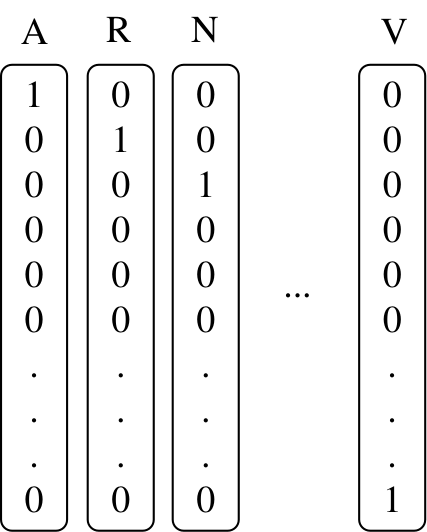
\includegraphics[width=0.3\textwidth]{../img/neoantigen/onehot}
			\caption{pMHC presentation process in MHC class I \cite{zhang2019application}.}		
		\end{figure}
	\end{frame}
	%-------------------------------------------------------
	%-------------------------------------------------------
	
	
	%-------------------------------------------------------
	%-------------------------------------------------------
	\begin{frame}{Input Encoding}{BLOSUM}	
		\begin{table}[]
			\tiny
			\centering
			\caption{BLOSUM62 matrix. Normally, it is used to represent amino acids numerically. Each amino acid is represented by a row.}
			\label{tab:blosum62}
			\setlength{\tabcolsep}{0.5em} % for the horizontal padding
			{\renewcommand{\arraystretch}{1.2}% for the vertical padding
				
				
				\begin{tabular}{lllllllllllllllllllll}
					& \textbf{C} & \textbf{S} & \textbf{T} & \textbf{P} & \textbf{A} & \textbf{G} & \textbf{N} & \textbf{D} & \textbf{E} & \textbf{Q} & \textbf{H} & \textbf{R} & \textbf{K} & \textbf{M} & \textbf{I} & \textbf{L} & \textbf{V} & \textbf{F} & \textbf{Y} & \textbf{W} \\
					\textbf{C} & 0          &            &            &            &            &            &            &            &            &            &            &            &            &            &            &            &            &            &            &            \\
					\textbf{S} & -1         & 4          &            &            &            &            &            &            &            &            &            &            &            &            &            &            &            &            &            &            \\
					\textbf{T} & -1         & 1          & 5          &            &            &            &            &            &            &            &            &            &            &            &            &            &            &            &            &            \\
					\textbf{P} & -3         & -1         & -1         & 7          &            &            &            &            &            &            &            &            &            &            &            &            &            &            &            &            \\
					\textbf{A} & 0          & 1          & 0          & -1         & 4          &            &            &            &            &            &            &            &            &            &            &            &            &            &            &            \\
					\textbf{G} & -3         & 0          & -2         & -2         & 0          & 6          &            &            &            &            &            &            &            &            &            &            &            &            &            &            \\
					\textbf{N} & -3         & -1         & 0          & -2         & -2         & 0          & 6          &            &            &            &            &            &            &            &            &            &            &            &            &            \\
					\textbf{D} & -3         & 1          & -1         & -1         & -2         & -1         & 1          & 6          &            &            &            &            &            &            &            &            &            &            &            &            \\
					\textbf{E} & -4         & 0          & -1         & -1         & -1         & -2         & 0          & 2          & 5          &            &            &            &            &            &            &            &            &            &            &            \\
					\textbf{Q} & -3         & 0          & -1         & -1         & -1         & -2         & 0          & 0          & 2          & 5          &            &            &            &            &            &            &            &            &            &            \\
					\textbf{H} & -3         & 0          & -2         & -2         & -2         & -2         & 1          & -1         & 0          & 0          & 8          &            &            &            &            &            &            &            &            &            \\
					\textbf{R} & -3         & -1         & -1         & -2         & -1         & -2         & 0          & -2         & 0          & 1          & 0          & 5          &            &            &            &            &            &            &            &            \\
					\textbf{K} & -3         & -1         & -1         & -1         & -1         & -2         & 0          & -1         & 1          & 1          & -1         & 2          & 5          &            &            &            &            &            &            &            \\
					\textbf{M} & -1         & 0          & -1         & -2         & -1         & -3         & -2         & -3         & -2         & 0          & -2         & -1         & -1         & 5          &            &            &            &            &            &            \\
					\textbf{I} & -1         & -2         & -1         & -3         & -1         & -1         & -4         & -3         & -3         & -3         & -3         & -3         & -3         & 1          & 4          &            &            &            &            &            \\
					\textbf{L} & -1         & -2         & -1         & -3         & -1         & -4         & -3         & -4         & -3         & -2         & -3         & -2         & -2         & 2          & 2          & 4          &            &            &            &            \\
					\textbf{V} & -1         & -2         & 0          & -2         & 0          & -3         & -3         & -3         & -2         & -2         & -3         & -3         & -2         & 1          & 3          & 1          & 4          &            &            &            \\
					\textbf{F} & -2         & -2         & -2         & -4         & -2         & -3         & -3         & -3         & -3         & -3         & -1         & -3         & -3         & 0          & 0          & 0          & -1         & 6          &            &            \\
					\textbf{Y} & -2         & -2         & -2         & -3         & -2         & -3         & -2         & -3         & -2         & -1         & 2          & -2         & -2         & -1         & -1         & -1         & -1         & 3          & 7          &            \\
					\textbf{W} & -2         & -3         & -2         & -4         & -3         & -2         & -4         & -4         & -3         & -2         & -2         & -3         & -3         & -1-        & -3         & -2         & -3         & 1          & 2          & 11        
				\end{tabular}
				
			}
		\end{table}
		
	\end{frame}
	%-------------------------------------------------------
	%-------------------------------------------------------
	
	
	
	%%%%%%%%%%%%%%%%%%%%%%%%%%%%%%%%%%%%%%%%%%%%%%%%%%%%%%%%%%%%%%%%%%%%%%%%%%%%%%%%%%%%%%%%%%%%%%%%%%%%%%%%%%%%%%%%
	%%%%%%%%%%%%%%%%%%%%%%%%%%%%%%%%%%%%%%%%%%%%%%%%%%%%%%%%%%%%%%%%%%%%%%%%%%%%%%%%%%%%%%
	\subsection{Transformers }
	%%%%%%%%%%%%%%%%%%%%%%%%%%%%%%%%%%%%%%%%%%%%%%%%%%%%%%%%%%%%%%%%%%%%%%%%%%%%%%%%%%%%%%%%%%%%%%%%%%%%%%%%%%%%%%%%
	%%%%%%%%%%%%%%%%%%%%%%%%%%%%%%%%%%%%%%%%%%%%%%%%%%%%%%%%%%%%%%%%%%%%%%%%%%%%%%%%%%%%%%
	
	
	
	%-------------------------------------------------------
	%-------------------------------------------------------
	\begin{frame}{Transformers}{}
		
		\begin{block}{}
			The \textbf{Transformer Neural Network} is a novel architecture that aims to solve sequence-to-sequence tasks while handling long-range dependencies with ease. It was proposed in the paper ``Attention Is All You Need'' \cite{vaswani2017attention}. 
		\end{block}
		
		\begin{block}{}
			\textbf{Bidirectional Encoder Representations from Transformers (BERT)} \cite{devlin2018bert} is a recent paper published by researchers at Google AI Language. It has caused a stir in the Machine Learning community by presenting state-of-the-art results in a wide variety of NLP tasks,
		\end{block}
		
	\end{frame}
	%-------------------------------------------------------
	%-------------------------------------------------------
	
	
	%-------------------------------------------------------
	%-------------------------------------------------------
	\begin{frame}{Transformers}{Transfer Learning}
		
		%\fontsize{12pt}{10pt}\selectfont
		\begin{table}[]
			
			\caption{List of pre-trained BERT models.}
			\setlength{\tabcolsep}{0.8em} % for the horizontal padding
			{\renewcommand{\arraystretch}{1.1}% for the vertical padding
				
				\begin{tabular}{lp{3cm}p{3cm}}
					\textbf{Model} & \textbf{Parameters}          & \textbf{Layers} \\ \hline
					TAPE           & 92M                          & 12                        \\
					ProtBert       & 420M                         & 30                        \\
					ESM1           & 43M, 85M y 670M              & 6, 12, and 34             \\
					ESM1-b         & 650M                         & 33                        \\
					ESM2           & 8M, 35M, 150M, 650M, 3B, 15B & 6, 12, 30, 33, 36, and 48
				\end{tabular}
				
			}
		\end{table}
		
		
	\end{frame}
	%-------------------------------------------------------
	%-------------------------------------------------------
	
	
	%-------------------------------------------------------
	%-------------------------------------------------------
	\begin{frame}{Transformers}{}
		
		%\fontsize{12pt}{10pt}\selectfont
		
		\begin{table}[]
			\caption{Transformers used for pMHC binding and presentation prediction.}
			\label{tab:transformes}
			\setlength{\tabcolsep}{0.5em} % for the horizontal padding
			{\renewcommand{\arraystretch}{1.1}% for the vertical padding
				
				\begin{footnotesize}
					\begin{tabular}{p{0.8cm}p{1.5cm}p{7.3cm}}
						\multicolumn{1}{l}{\textbf{Year}}                                   & \textbf{Name}                       & \textbf{Model}     \\  \hline
						
						2022\cite{zhang2022hlab}&	\textbf{HLAB}&	BERT from ProtBert pre-trained model followed by a BiLSTM with attention mechanism.	\\
						
						2022\cite{wang2022mhcroberta}          & MHC RoBERTa             &  RoBERTa  pre-trained and followed by 12 multi-head SA and a FC layers, it outperformed NetMHCPan 3.0.                                                                                          \\
						2022\cite{chu2022transformer}          & \textbf{TransPHLA}                     & It used SA mechanism based on four blocks, it slightly outperformed NetMHCpan4.1 and is faster making predictions.\\
						
						2021\cite{gasser2021interpreting}  & ImmunoBERT                              & BERT from TAPE pre-trained followed by a linear layer. Authors claimed that N-terminal and C-terminals are highly relevant after analysis with SHAP and LIME.   \\
						
						2021\cite{cheng2021bertmhc}             & BERTMHC                            & BERT from TAPE pre-trained followed by a linear layer. It outperformed NetMHCIIpan3.2 and PUFFIN.   \\
						
					\end{tabular}
				\end{footnotesize}
			}
		\end{table}
		
		
	\end{frame}
	%-------------------------------------------------------
	%-------------------------------------------------------
	
	

	
	%%%%%%%%%%%%%%%%%%%%%%%%%%%%%%%%%%%%%%%%%%%%%%%%%%%%%%%%%%%%%%%%%%%%%%%%%%%%%%%%%%%%%%%%%%%%%%%%%%%%%%%%%%%%%%%%
	%%%%%%%%%%%%%%%%%%%%%%%%%%%%%%%%%%%%%%%%%%%%%%%%%%%%%%%%%%%%%%%%%%%%%%%%%%%%%%%%%%%%%%
	\subsection{Limitations }
	%%%%%%%%%%%%%%%%%%%%%%%%%%%%%%%%%%%%%%%%%%%%%%%%%%%%%%%%%%%%%%%%%%%%%%%%%%%%%%%%%%%%%%%%%%%%%%%%%%%%%%%%%%%%%%%%
	%%%%%%%%%%%%%%%%%%%%%%%%%%%%%%%%%%%%%%%%%%%%%%%%%%%%%%%%%%%%%%%%%%%%%%%%%%%%%%%%%%%%%%
	
	%-------------------------------------------------------
	%-------------------------------------------------------
	\begin{frame}{Limitations}{}
		
		\begin{block}{}
			They ignored Posttranslational modifications (PTMs) such as phosphorylation, glycosylation, and deamidation, which influence the specificity of MHC binding and presentation and several aspects of the biology underlying pMHC presentation are poorly understood. Furthermore, to get accurate results for neoantigen detection, we need to integrate pMHC-TCR studies. 
		\end{block}
		
		\begin{block}{}
			Another limitations are related to high computing requirements for training BERT architectures. For instance, the biggest ESM2 model has 15 billion parameters.
		\end{block}
		
	\end{frame}
	%-------------------------------------------------------
	%-------------------------------------------------------
	
	%%%%%%%%%%%%%%%%%%%%%%%%%%%%%%%%%%%%%%%%%%%%%%%%%%%%%%%%%%%%%%%%%%%%%%%%%%%%%%%%%%%%%%%%%%%%%%%%%%%%%%%%%%%%%%%%
	%%%%%%%%%%%%%%%%%%%%%%%%%%%%%%%%%%%%%%%%%%%%%%%%%%%%%%%%%%%%%%%%%%%%%%%%%%%%%%%%%%%%%%
	\subsection{Future works }
	%%%%%%%%%%%%%%%%%%%%%%%%%%%%%%%%%%%%%%%%%%%%%%%%%%%%%%%%%%%%%%%%%%%%%%%%%%%%%%%%%%%%%%%%%%%%%%%%%%%%%%%%%%%%%%%%
	%%%%%%%%%%%%%%%%%%%%%%%%%%%%%%%%%%%%%%%%%%%%%%%%%%%%%%%%%%%%%%%%%%%%%%%%%%%%%%%%%%%%%%
	
	%-------------------------------------------------------
	%-------------------------------------------------------
	\begin{frame}{Future works}{}
		
		\begin{block}{}
			Future work could include the use of transfer learning from ESM1-b \cite{rives2021biological} and ESM2 \cite{lin2023evolutionary}. 
		\end{block}
		
		\begin{block}{}
			Moreover, there is pHLA3D, a dataset of 3D structures of the alpha/beta chains and peptides of MHC-I proteins; it opens new perspectives for studying pMHC prediction. 
		\end{block}
		
	\end{frame}
	%-------------------------------------------------------
	%-------------------------------------------------------
	

	
	%-------------------------------------------------------
	%-------------------------------------------------------
	\begin{frame}[allowframebreaks, noframenumbering]
		\frametitle{References}
		%\bibliographystyle{amsalpha}
		\bibliographystyle{IEEEtran}
		\bibliography{../bibliography_thesis.bib}
	\end{frame}
	%-------------------------------------------------------
	%-------------------------------------------------------
	
	%-------------------------------------------------------
	%-------------------------------------------------------
	\if\mycmd1 % MY THEME
	\1{
		{\1
			\begin{frame}[plain,noframenumbering]
				%\finalpage{Thank you}
				\begin{figure}[]
					\centering
					
\includegraphics[width=\textwidth,height=0.7\textheight,keepaspectratio]{../img/question.png}
					%\label{img:mot2}
					%\caption{Image example in 2 gray levels.}
				\end{figure}
		\end{frame}}
		\else % CS THEME
		\begin{frame}{Questions?}
			\begin{figure}[]
				\centering
				
\includegraphics[width=\textwidth,height=0.7\textheight,keepaspectratio]{../img/question.png}
				%\label{img:mot2}
				%\caption{Image example in 2 gray levels.}
			\end{figure}
			
		\end{frame}
		\fi
		%-------------------------------------------------------
		%-------------------------------------------------------
		
		
	\end{document}